
\documentclass[xcolor=dvipsnames]{beamer} 
\usecolortheme[named=BurntOrange]{structure}
\usetheme{shadow} 
\usepackage{adjustbox}
\usepackage{graphicx}
\usepackage{multicol}
\useoutertheme{infolines}


\author{}
\institute{UCSB Computer Science}
\title{CS290G : Course Project}
\date{\today}
\section{Cryptographic Engineering}
\subsection{Implementation of D-H Key Exchange on UDOO}

\begin{document}

\begin{frame}
\begin{center}
\textbf{\Large An efficient implementation of Diffie-Hellman key exchange protocol on UDOO}  \\[1em]
Sachin Rathod and Sahaj Biyani \\
\url{{rathod,sahajbiyani}@cs.ucsb.edu} \\[1em]

\end{center}
\end{frame}

\begin{frame}{Diffie-Hellman Key Exchange}
\begin{itemize}
\item How can two parties agree on a secret value when all of their
messages might be overheard by an eavesdropper?
\item The Diffie-Hellman [1] key agreement protocol (1976) was the first
practical method for establishing a shared secret over an unsecured
communication channel.
\item  The point is to agree on a key that two parties can use for a
symmetric encryption, in such a way that an eavesdropper cannot
obtain the key.
\item The Diffie-Hellman algorithm accomplishes this, and is still
widely used.
\medskip
\end{itemize}
\end{frame}

\begin{frame}{Diffie-Hellman Algorithm Analogy}
\centering
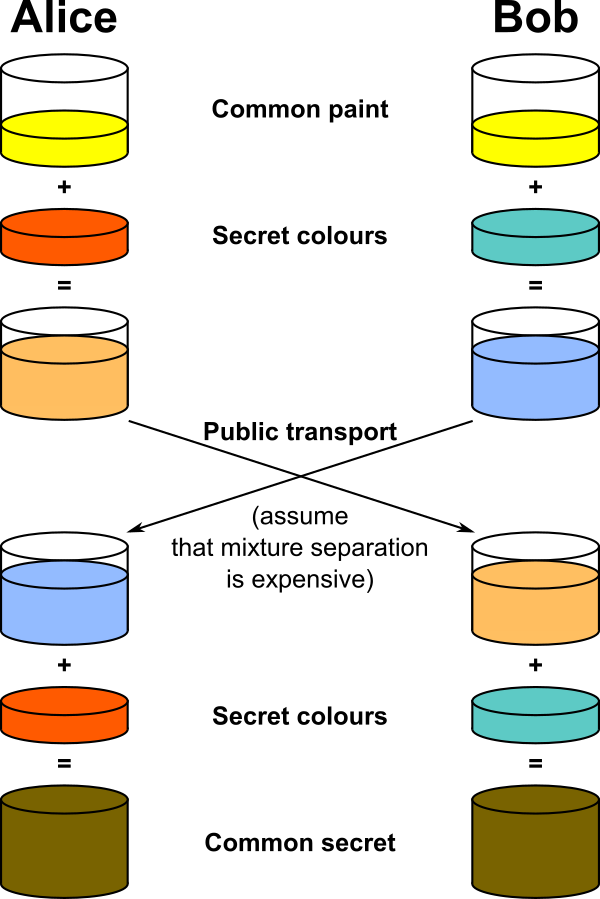
\includegraphics[scale=0.2]{dh.png}
\end{frame}

\begin{frame}{Diffie-Hellman Algorithm}
Steps in the Algorithm:
\begin{enumerate}
\item Alice and Bob agree on a prime number $p$ and a base $g$.
\item Alice chooses a secret number $a$, and sends Bob ($g^a$  mod $p $)
\item Bob chooses a secret number $b$, and sends Alice ($g^b$  mod $p $)
\item Alice computes (($g^b$  mod $p )^a$ mod $p$)
\item Bob computes (($g^a$  mod $p )^b$ mod $p$)
\end{enumerate}
\end{frame}

\begin{frame}{Implementation Methods}
We tried different exponentiation methods to compute the key values to compare their performance on different platforms.\\
\medskip
Three methods of exponentiation:\\
\begin{enumerate}
\item Binary Exponentiation (Implemented)
\item Montgomery Exponentiation (Implemented)
\item OpenSSL (Used from library)
\end{enumerate}
\end{frame}

\begin{frame}{Implementation}
\begin{itemize}
\item For managing arbitrary length numbers, we used OpenSSL's BIGNUM structure [2] and its library functions.
\medskip
\item This library performs operations on integers of arbitrary size. The operations include arithmetic (add, multiply etc.), comparison, conversion to different formats etc.
\end{itemize}
\end{frame}

\begin{frame}{Binary Exponentiation Method}
One of the methods we used for analysis is binary exponentiation. The binary exponentiation method is explained by the following algorithm:\\
\medskip
\begin{tabular}{rl}
Input: & $M,e,n.$\\
Output: & $C = M^e \ mod \ n.$\\
Step 1. &$if \ e_{k-1} = 1 \ then \ C=M \ else \ C=1$\\
Step 2. &$if \ i = k-2 \ downto \ 0$\\
2a. & \hspace{5mm}$C = C.C \ (mod \ n )$\\
2b.  & \hspace{5mm}$ if \ e_i=1 \ then \ C=C.M \ (mod \ n) $\\
Step 3. & return $C$\\
\end{tabular}
\end{frame}

\begin{frame}{Montgomery Exponentiation Method}
Another method we used for analysis is montgomery exponentiation. The montgomery exponentiation method is explained by the following algorithm:\\
\medskip
\textbf{function} MonPro$(\bar a,\bar b)$\\
\begin{tabular}{rl}
Step 1. &$t = \bar a. \bar b$\\
Step 2. &$m=t.n' \ mod \ r$\\
Step 3. & $u = (t + m.n ) / r$\\
Step 4.  & $\textbf{if} \  u\geq n \ \textbf{then return} \ u-n$ \\
& \hspace{13mm} \textbf{else return} $ u $\\
\end{tabular}
\end{frame}


\begin{frame}{Montgomery Exponentiation Method}
\textbf{function} ModExp$(M,e,n)$ \{ n is odd \}\\
\begin{tabular}{rl}
Step 1. & Compute $n'$ using Euclid's algorithm\\
Step 2. & $\bar M = M.r \ mod \ n$\\
Step 3. & $\bar C = 1.r \ mod \ n$\\
Step 4.  & $ \textbf{for} \  i=k-1 \  \textbf{down to}  \ 0 \ \textbf{do} $\\
Step 5. & \hspace{5mm} $\bar C = MonPro(\bar C, \bar C)$\\
Step 6. & \hspace{5mm} $\textbf{if} \ e_i=1 \ \textbf{then} \bar \ C = MonPro(\bar M, \bar C) $\\
Step 7. & $C = MonPro(\bar{C},1)$\\
Step 8. & return $C$\\
\end{tabular}
\end{frame}

\begin{frame}{Hardware Specifications: UDOO Board}
Results are compared between UDOO board and standard PC with following configurations:\\
\medskip
\centering
\adjustbox{max height=\dimexpr\textheight-5.5cm\relax,max width=\textwidth} {
\begin{tabular}{| c | c | c |}
\hline
& UDOO & PC\\
\hline
CPU & 1 x [ARMv7 Processor rev 10 (v7l)] &  4 x [Intel(R) Core(TM) i5-3337U CPU @ 1.80GHz]\\
\hline
Physical Memory & 800 MB & 3.7 GB\\
\hline
OS & Ubuntu 12.04 32-bit & Ubuntu 14.04 64-bit\\
\hline
\end{tabular}
}
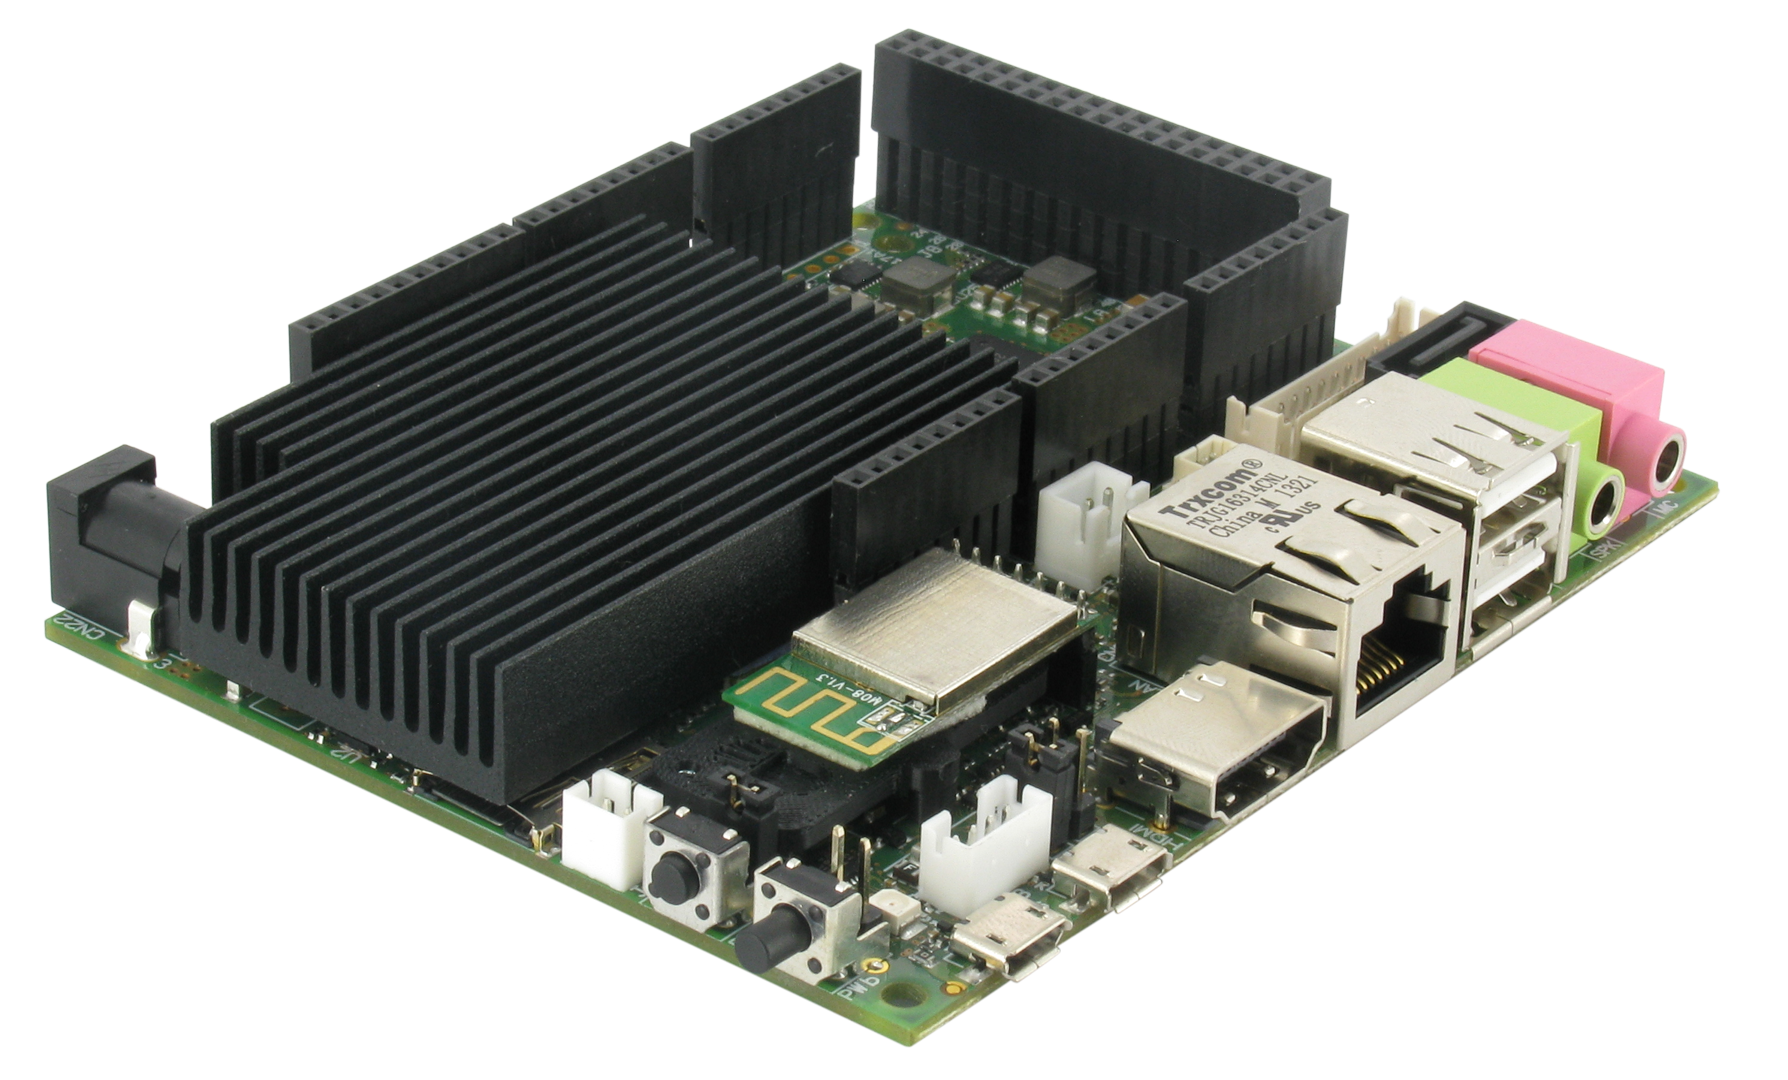
\includegraphics[scale=0.09]{udoo}\\
\end{frame}

\begin{frame}{Diffie-Hellman Parameters}
\begin{itemize}
\item Prime $p$ and generator $g$:\\
\begin{enumerate}
\item IETF standard 1024 and 2048-bit primes and corresponding generators (having 160-bit and 224-bit prime order subgroups). RFC5114 [3]
\medskip
\item Random 'safe' primes generated using OpenSSL library having given number of bits and generator $g$ is taken as $5$). (Safe primes are of the form $2p+1$, where $p$ is also prime) 
\end{enumerate}
\item Safe primes are of the form $2p+1$, where p is also prime. Safe primes offers security against Pohlig and Hellman attacks, but require more computation.
\item Parameters $a$ and $b$ :
random primes with given number of bits
\end{itemize}
\end{frame}

\begin{frame}{Results on UDOO}

Avg time required for key generation on UDOO (in seconds):\\
\medskip
\adjustbox{max height=\dimexpr\textheight-5.5cm\relax,max width=\textwidth} {
\begin{tabular}{|c | c | c | c |}
\hline
Key-size (bits) & Binary Exponentiation & Montgomery Exponentiation & OpenSSL Exponentiation\\
\hline
256 & 0.005414833 & 0.009804000 & 0.001707833 \\
\hline
512 & 0.023968332 & 0.047772333 & 0.008993666\\
\hline
1024 & 0.148043826 & 0.284063160 & 0.058445834\\
\hline
2048 & 0.294208169 & 0.564812660 & 0.114655666\\
\hline
\end{tabular}
}
\end{frame}


\begin{frame}{Comparing UDOO and PC}
Avg time required for key generation (in seconds):\\
\medskip
\adjustbox{max height=\dimexpr\textheight-5.5cm\relax,max width=\textwidth} {
\begin{tabular}{| l | c | c | c |}
\hline
Key-size (bits) & Binary Exponentiation & Montgomery Exponentiation & OpenSSL Exponentiation\\
\hline
1024 [UDOO] & 0.148043826 & 0.284063160 & 0.058445834\\
\hline
1024 [PC] & 0.007844172 & 0.018422132 & 0.001439296\\
\hline
2048 [UDOO] & 0.294208169 & 0.564812660 & 0.114655666\\
\hline
2048 [PC] & 0.015397863 & 0.036434080 & 0.002855158\\
\hline
\end{tabular}
}
\end{frame}

\begin{frame}{Conclusions}
\noindent D-H key generation performance:
\begin{itemize}
\item Binary exponentiation 2-3 times faster than Montgomery exponentiation.
\item OpenSSL implementation of exponentiation is ~3 times faster than our binary exponentiation.
\item This could be because OpenSSL implementation is highly efficient than our implementation.
\end{itemize}
\end{frame}

\begin{frame}{Key Learnings from the Project}
\noindent We learnt a lot from this project. Some of the learnings are as follows:
\begin{itemize}
\item Hands-on development on the UDOO platform.
\item The use of OpenSSL library for handling arbitrary length integer operations in C programming language.
\item The implementation of security protocols and operations in secure and efficient manner.
\end{itemize}
\end{frame}

\begin{frame}{Future Work}

\noindent Future iterations of this project can include: 
\begin{itemize}
\item Improving efficiency of Montgomery exponentiation implementation for UDOO board.
\item Using the key exchange implementation to communicate messages between remote clients and testing its security.
\end{itemize}
\end{frame}

\begin{frame}{References}
\begin{tabular}{r p{85mm}}
\lbrack1\rbrack  & Diffie, W.; Hellman, M. (1976). "New directions in cryptography". IEEE Transactions on Information Theory 22 (6): 644 - 654. doi:10.1109/TIT.1976.1055638\\
\lbrack2\rbrack \  & Open SSL - Cryptography and SSL/TLS Toolkit \lbrack https://www.openssl.org/\rbrack\\
\medskip
\lbrack3\rbrack \  & IETF Standard RFC5114  \lbrack http://tools.ietf.org/html/rfc5114\rbrack\\
\medskip

\end{tabular}
\end{frame}

\end{document}
